
\documentclass{article}

\usepackage{color}
\usepackage{epsfig}
\usepackage{amssymb}
\usepackage{listings}
\usepackage{textpos}
\usepackage{amsmath}

%\usetheme{Berlin}
%\usecolortheme{seahorse}
%\usefonttheme{professionalfonts}

\begin{document}

  \section*{Homework 2}

  {\bf Due on 2 November}\\

  A $d$-ary function $f$ is convex if and only if the following inequality holds for each pair of $d\times 1$ vectors $x_1,x_2\in \mathbb{R}^d$ and each constant $\alpha\in[0,1]$:
\[
f(\alpha x_1 + (1-\alpha)x_2) \leq \alpha f(x_1) + (1-\alpha) f(x_2).
\]

\centerline{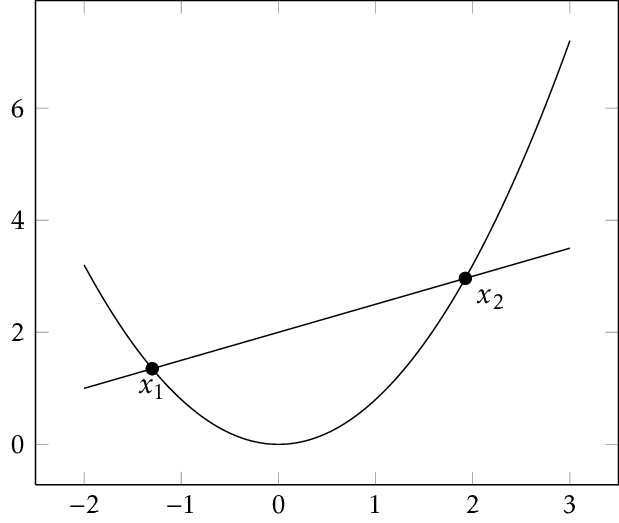
\includegraphics[height=5cm]{convexfun.png}}

\noindent
The intuition is that between $x_1$ and $x_2$, the function $f$ lies {\em below} a straight line from $x_1$ to $x_2$, as in the above figure.\\

Assuming that the two $d$-ary functions $f$ and $g$ are convex, show that the following $d$-ary functions are also convex:
\begin{enumerate}
\item $h(x) = a\cdot f(x)$, for any constant $a>0$.
\item $h(x) = f(x) + g(x)$.
\item $h(x) = \max(f(x),g(x))$.
\item $h(x) = f(Ax + b)$, for any $d\times d$ matrix $A$ and $d\times 1$ vector $b$.
\end{enumerate}
Hint: to show convexity, you need to show that the inequality above holds for the different functions and any choice of $x_1$, $x_2$ and $\alpha\in[0,1]$. Since $f$ and $g$ are assumed convex, we know that the inequality {\em does} hold for those functions.

\end{document}
